\chapter{第五部分 近代物理}
\section{第二章 狭义相对论}

\textbf{1}
一艘宇宙飞船以0.8c的速度于中午飞经地球，此时飞船上和地球上的观察者都把自己的时钟拨到12点。

\begin{enumerate}
\item 按飞船上的时钟于午后 12 点 30 分飞经一星际宇航站, 该站相对地球固定, 其时钟指示的是地球时间. 试问按宇航站的时钟飞船何时到达该站?
\item 试问按地球上的坐标测量,宇航站离地球多远?
\item 于飞船时间午后 12 点 30 分从飞船向地球发送无线电信号, 试问地球上的观察者何时 (按地球时间) 接到信号?
\item 若地球上的观察者在接收到信号后立即发出回答信号, 试问飞船何时(按飞船时间)接收到回答信号?
\end{enumerate}
\vfill

\textbf{2}
如近图2-2-1所示，有一均匀带电的正方形绝缘线框ABCD，每边边长为 $L$ ，线框上串有许多带电小球(看成质点)，每个小球的带电量为 $q$ ，每边的总带电量为零(即线框的带电量和各小球的带电量互相抵消). 今各小球相对线框以速率 $u$ 沿绝缘线作匀速运动, 在线框参考系中测得相邻两小球的间距为 $a (\ll L)$ . 线框又沿 $AB$ 边以速率 $v$ 在自身平面内相对 $S$ 系作匀速运动. 在线框范围内存在一均匀电场 $\pmb{E}$ , 其方向与线框平面的倾角为 $\theta$ . 考虑相对论效应, 试在 $S$ 系中计算以下各量.

\begin{enumerate}
\item 线框各边上相邻两小球的间距 $a_{AB}, a_{BC}, a_{CD}, a_{DA}$ .
\item 线框各边的净电量 $Q_{AB}, Q_{BC}, Q_{CD}, Q_{DA}$ .
\end{enumerate}

\begin{figure}[htbp]
\centering
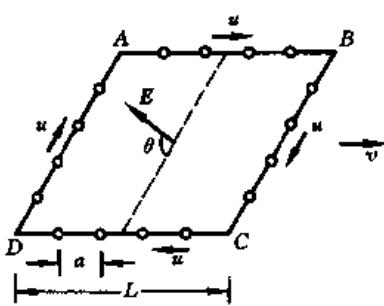
\includegraphics[width=0.6\textwidth]{figures/近图2-2-1.jpg}
\caption{近图2-2-1}
\end{figure}

\begin{enumerate}
\setcounter{enumi}{2}
\item 线框和小球系统所受的电力矩大小.
\item 线框和小球系统的电势能。
\end{enumerate}
\vfill

\newpage
\textbf{3}
如近图2-3-1所示，在某恒星参考系 $S$ 中，飞船A和飞船B以相同速率 $\beta c(c$ 为真空中的光速)作匀速直线运动。飞船 $A$ 的运动方向与 $+x$ 方向一致，而飞船 $B$ 的运动方向与 $-x$ 方向一致，两飞船轨迹之间的垂直距离为 $d$ 。当 $A$ 和 $B$ 靠得最近时，从 $A$ 向 $B$ 发出一细束无线电联络信号．

试问:
\begin{enumerate}
\item 为使 B 能接收到信号, A 中的宇航员认为发射信号的方向应与自己的运动方向之间成什么角?
\item 飞船 B 接收到信号时, B 中的宇航员认为自己与飞船 A 相距多少?
\end{enumerate}
\vfill

\textbf{4}
如近图2-4-1所示，平面反射镜 $M$ 固定在 $S'$ 系的 $x'y'$ 平面内，其法线方向与 $x'$ 轴一致。反射镜相对 S 系以速度 v 沿法线方向作平移运动。试求光在反射镜上反射时，入射角与反射角所遵从的关系。
\vfill

\newpage
\textbf{5}
如近图2-5-1所示，由介质1和介质2构成一界面，两介质的折射率为 $n_1$ 和 $n_2$ ，界面的法线与 S 系的 x 轴一致。现界面相对 S 系中的观察者以速度 v 沿法线作匀速平行运动，在 S 系中入射光以入射角 $\theta_{i}$ 从介质 1 向界面入射，反射角和折射角分别用 $\theta_{r}$ 和 $\theta_{t}$ 表示。试导出 S 系中的观察者观测到的反射角和折射角与入射角的关系。

\begin{figure}[htbp]
\centering
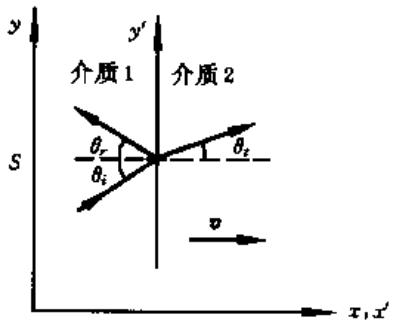
\includegraphics[width=0.6\textwidth]{figures/近图2-5-1.jpg}
\caption{近图2-5-1}
\end{figure}
\vfill

\textbf{6}
如近图2-6-1所示，惯性系 $S$ 和 $S'$ 的对应坐标轴互相平行， $S'$ 系相对 $S$ 系以速度 $v$ 沿 $+z$ 方向运动。 $S$ 系与某星体连结在一起，两坐标系的原点 $O$ 和 $O'$ 的间距远小于到其他星体的距离。假定在 $O$ 处的观察者看到的其他星体的个数各向同性分布，即在任何方向上单位立体角内测得的星体个数 $N$ 为常量。试求在 $O'$ 处的观察者看到的星体个数的分布。
\vfill

\newpage
\textbf{7}
如近图2-8-1所示，一单色点光源在其静止的参考系 $S^{\prime}$ 中向四周均匀地辐射光能量，其发光强度为 $I_0$ 。当该点光源相对 $S$ 系中的观察者以速度 $\pmb{\upsilon}$ 运动时，测得的发光强度将随观察方位而变。设 $S$ 系中的观察者位于 $P$ 点，观察方向与点光源运动方向之间的夹角用 $\theta$ 表示。试求 $S$ 系中测得的发光强度 $I$ 与角 $\theta$ 的关系。

\begin{figure}[htbp]
\centering
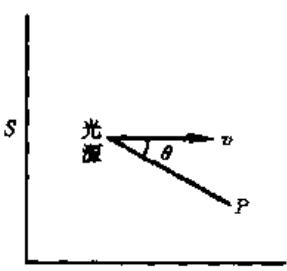
\includegraphics[width=0.6\textwidth]{figures/近图2-7-1.jpg}
\caption{近图2-7-1}
\end{figure}
\vfill

\textbf{8}
如近图2-8-1所示，光源S向全反射体 $S'$ 发射一束平行光，发光功率为 $P_{0}$ 。设 $S'$ 以匀速率v沿其法线方向朝S运动。试求S接收到的反射光功率。
\begin{center}
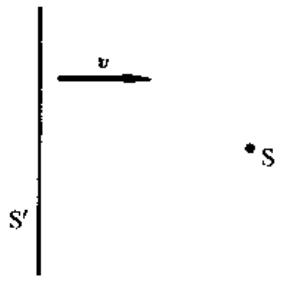
\includegraphics[width=0.3\textwidth]{figures/近图2-8-1.jpg}
\end{center}
\vfill

\newpage
\textbf{9}
如近图2-10-1所示,光源静止于S系中,某色散介质相对S系沿x方向以速度v运动.试问,对S 系中的观察者而言, 光在介质中的传播速度是多少? 已知光在静止介质中的波长为 $\lambda$ , 相应的折射率为 n, 介质的色散率为 $\frac{dn}{d\lambda}$ . 计算时只取一级近似。
\begin{center}
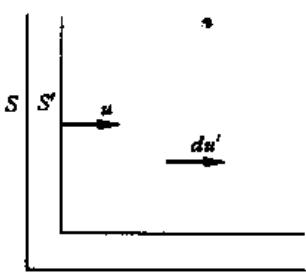
\includegraphics[width=0.25\textwidth]{figures/近图2-10-1.jpg}
\end{center}
\vfill

\textbf{10}
宇宙飞船从地球出发沿直线飞向某恒星，恒星距地球 $r = 3 \times 10^{4} \mathrm{l}. \mathrm{y}$ . (光年). 对每一瞬时都与飞船连结在一起的坐标系来讲，前一半路程作匀加速直线运动，加速度 $a' = 10 \mathrm{~m} / \mathrm{s}^{2}$ ，后一半路程以数值相同的加速度作匀减速运动。试问在飞船上测量，整个旅程经历了多少时间？计算时只取一级近似。
\vfill

\newpage
\textbf{11}
太空火箭(包括燃料)的初始质量为 $M_0$ ，从静止起飞，向后喷出的气体相对火箭的速度 $u$ 为常量。任意时刻火箭速度(相对地球)为 $v$ 时火箭的静止质量为 $m_0$ 。忽略引力影响。试求比值 $\frac{m_0}{M_0}$ 与速度 $v$ 之间的关系。
\vfill

\textbf{12}
光子火箭从地球起程时初始静止质量(包括燃料)为 $M_0$ ，向相距为 $R = 1.8\times 10^{6}\mathrm{l.y.}$ （光年）的远方仙女座星云飞行．要求火箭在25年(火箭时间)后到达目的地，引力影响不计．

\begin{enumerate}
\item 忽略火箭加速和减速所需时间, 试问火箭的速度应为多大?
\item 设到达目的地时火箭静止质量为 $M_{0}^{\prime}$ , 试问 $\frac{M_{0}}{M_{0}^{\prime}}$ 的最小值是多少?
\end{enumerate}
\vfill

\newpage
\textbf{13}
光子火箭的飞行目的地为银河系中心，已知银河系中心离地球的距离为 $R = 3.4 \times 10^{4} \mathrm{l.y}$ （光年）。火箭在前一半旅程以加速度 $a' = 10 \mathrm{~m} / \mathrm{s}^{2}$ （相对火箭的静止系）作匀加速运动，而后一半旅程则以同样的加速度作减速运动。火箭到达目的地时的静止质量 $M_{0}' = 1.0 \times 10^{6} \mathrm{~kg}$ 。试问火箭发动机在开始发射时至少需要多大功率？
\vfill

\textbf{14}
$\mu$ 子的电量 $q = -e(e = 1.6\times 10^{-19}\mathrm{C})$ ，静止质量 $m_0 = 100\mathrm{MeV} / c^2$ ，静止时的寿命 $\tau_0 = 10^{-6}\mathrm{s}$ .设在地球赤道上空离地面高度为 $h = 10^{4}\mathrm{m}$ 处有一 $\mu$ 子以接近于真空中光速的速度垂直向下运动.

\begin{enumerate}
\item 试问此 $\mu$ 子至少应有多大总能量才能到达地面？
\item 若把赤道上空 $10^{4} \mathrm{~m}$ 高度范围内的地球磁场看作匀强磁场，磁感应强度 $B = 10^{-4} \mathrm{T}$ ，磁场方向与地面平行。试求具有第1问所得能量的 $\mu$ 子在到达地面时的偏离方向和总的偏转角。
\end{enumerate}
\vfill

\newpage
\textbf{15}
某电子显微镜电子的加速电压 $U = 512\mathrm{kV}$ ，先将静止电子加速，加速后的电子束进入非均匀磁场区，非均匀磁场由一系列线圈 $L_{1}, L_{2}, \dots, L_{N}$ 产生，各线圈中的电流强度分别为 $i_{1}, i_{2}, \dots, i_{N}$ 。电子在非均匀磁场区沿一确定轨道 $T$ 运动。今欲将该电子显微镜改装成质子显微镜，以 $-U$ 加速静止质子，要求质子进入非均匀磁场区后沿着与电子完全相同的轨道运动，则各线圈中的电流 $i_{1}', i_{2}', \dots, i_{N}'$ 与原电流 $i_{1}, i_{2}, \dots, i_{N}$ 应有何种关系？
\vfill

\textbf{16}
一粒子的静止质量为 $m_0$ ，以初速 $v_0$ 开始沿 $x$ 轴方向运动，在运动期间始终受到一个指向 $y$ 轴方向的恒力 $\pmb{F}$ 的作用。试证明，任意时刻粒子的两个速度分量为

$$
v _ {x} = \frac {v _ {0}}{\sqrt {1 - \frac {v _ {0} ^ {2}}{c ^ {2}}}} \sqrt {\frac {c ^ {2}}{c ^ {2} + k}}
$$

$$
v _ {y} = \frac {F t}{m _ {0}} \sqrt {\frac {c ^ {2}}{c ^ {2} + k}}
$$

式中

$$
k = \frac {v _ {0} ^ {2}}{1 - \frac {v _ {0} ^ {2}}{c ^ {2}}} + \left(\frac {F t}{m _ {0}}\right) ^ {2}
$$

并证明，当 $t \to \infty$ 时，速率 $v \to c, v_x \to 0$ .
\vfill

\newpage
\textbf{17}
相对论性粒子。

在狭义相对论里,一个质量为 $m_{0}$ 的自由粒子的能量 E 和动量 p 之间的关系为

$$
E = (p ^ {2} c ^ {2} + m _ {0} ^ {2} c ^ {4}) ^ {\frac {1}{2}} = m c ^ {2}
$$

当这样的粒子受到一个保守力作用时, 其总能量, 即 $(p^2 c^2 + m_0^2 c^4)^{\frac{1}{2}}$ 与势能之和是守恒的. 如果粒子的能量非常高, 则它的静止能量可以忽略, 这样的粒子叫做极端相对论性粒子.

\begin{enumerate}
\item 考虑一个能量极高的作一维运动的粒子(忽略静止能量), 受到一个大小为 $f =$ 常量的向心吸引力的作用. 设开始时 $(t = 0)$ 粒子处于力心 $(x = 0)$ , 具有初始动量 $p_0$ . 试在 $(p, x)$ 图上 (动量-空间坐标图) 和在 $(x, t)$ 图上 (坐标-时间图) 分别画出粒子运动的图象, 要求至少画一个运动周期, 标明各转折点的坐标 (用所给参数 $p_0$ 和 $f$ 表示), 并在 $(p, x)$ 图上用箭头指示出运动过程的方向.

\item 介子是一种由两个夸克构成的粒子。介子的静止质量 $M$ 等于两夸克系统的总能量除以 $c^2$ .
考虑一个关于静止介子的一维模型, 其中两个夸克沿着 $x$ 轴运动, 它们之间存在着一个常数吸引力, 大小为 $f$ , 并假定它们可以自由地互相穿透. 在分析夸克的高能运动时, 它们的静止质量可以忽略. 设开始计时时 $(t = 0)$ 两夸克都在 $x = 0$ 处. 试在 $(x, t)$ 图上和 $(p, x)$ 图上指示出运动的方向, 并求出两夸克之间的最大距离.

\item 上面第2问中所用的参考系记为 $S$ ，今有一实验室参考系 $S'$ ， $S'$ 相对于 $S$ 以恒定速度 $v = 0.6c$ 沿负 $x$ 方向运动。两参考系的坐标这样选择，即使得 $S$ 系中的 $x = 0$ 点与 $S'$ 系中的 $x' = 0$ 点在 $t = t' = 0$ 时重合。试在 $(x', t')$ 图上画出两夸克的运动图象，标出转折点的坐标（用 $M, f$ 和 $c$ 表示），并给出 $S'$ 系观察到的两夸克之间的最大距离。

在 S 系和 $S'$ 系中观察到的粒子的坐标之间的关系由洛伦兹变换决定，即

$$
\begin{array}{r l} x ^ {\prime} & = r (x + \beta c t) \\ t ^ {\prime} & = r (t + \frac {\beta x}{c}) \end{array}
$$

式中 $\beta=\frac{v}{c}, r=\frac{1}{\sqrt{1-\beta^{2}}}, v$ 是 S 系相对于 $S'$ 系的速度。

\item 已知一介子, 其静止能量为 $Mc^2 = 140\mathrm{MeV}$ , 相对于实验室系 $S'$ 的速度为 $0.60c$ . 试求出它在 $S'$ 系中的能量.
\end{enumerate}
\vfill

\textbf{18}
星体一旦形成黑洞，那么其表面的光子都不可能离开黑洞外逸。设星体质量具有球对称分布，总质量为 $M$ 。试用狭义相对论估算它刚好能成为黑洞的半径。
\vfill

\newpage
\textbf{19}
引力红移和恒星质量的测定。

\begin{enumerate}
\item 频率为 $f$ 的一个光子具有惯性质量 $m$ , 此质量由光子的能量确定。在此假定下光子也有引力质量, 量值等于惯性质量。与此相应, 从一颗星球表面向外发射出的光子, 逃离星球引力场时, 便会损失能量。
试证明,初始频率为 f 的光子从星球表面到达无穷远处,若将它的频移(频率增加量)记为
$\Delta f$ ，则当 $\Delta f\ll f$ 时，有

$$
\frac {\Delta f}{f} \approx - \frac {G M}{R c ^ {2}}
$$

式中 $G$ 为引力常量， $R$ 为星球半径， $c$ 为真空光速， $M$ 为星球质量。这样，在距星球足够远处对某条已知谱线频率红移的测量，可用来测出比值 $\frac{M}{R}$ ，如果知道了 $R$ ，星球的质量 $M$ 便可确定。

\item 在一项太空实验中发射出一艘无人驾驶的宇宙飞船, 欲测量银河系中某颗恒星的质量 $M$ 和半径 $R$ . 宇宙飞船径向地接近目标时, 可以监测到从星球表面 $\mathrm{He}^{+}$ 离子发射出的光子对飞船实验舱内的 $\mathrm{He}^{+}$ 离子束进行共振激发. 共振吸收的条件是飞船 $\mathrm{He}^{+}$ 离子朝着星球的速度必须与光子引力红移严格地相适应. 共振吸收时的飞船 $\mathrm{He}^{+}$ 离子相对星球的速度 $v$ (记为 $v = \beta c$ ), 可随着飞船到星球表面最近距离 $d$ 的变化而进行测量, 实验数据在下面表格中给出. 请充分利用这些数据, 试用作图法求出星球的半径 $R$ 和质量 $M$ . 解答中不必进行误差估算。

\begin{center}
\begin{tabular}{|c|c|c|c|c|c|}
\hline
速度性参量 $\beta = \frac{v}{c}$ ( $10^{-5}$ ) & 3.352 & 3.279 & 3.195 & 3.077 & 2.955 \\
\hline
到星体表面距离 $d/(10^{8}\,\mathrm{m})$ & 38.90 & 19.98 & 13.32 & 8.99 & 6.67 \\
\hline
\end{tabular}
\end{center}

\item 为在本实验中确定 R 和 M，通常需要考虑因发射光子时离子的反冲造成的频率修正（热运动对发射谱线仅起加宽作用，不会使峰的分布移位，因此可以假定热运动的全部影响均已被审查过了）.
\begin{enumerate}
\item 令 $\Delta E$ 为原子(或者说离子)在静止时的两个能级差, 假定静止原子在能级跃迁后产生一个光子并形成一个反冲原子. 考虑相对论效应, 试用能级差 $\Delta E$ 和初始原子静止质量 $m_0$ 来表述发射光子的能量 $hf$ .
\item 现在, 试对 $\mathrm{He}^{+}$ 离子这种相对论频移比值 $\left(\frac{\Delta f}{f}\right)$ 反冲作出数值计算.
\end{enumerate}
计算结果应当得出这样的结论,即反冲频移远小于第2问中得出的引力红移.

计算用常量：

真空光速 $c=3.0\times10^{8}$ m/s, He 的静质量 $m_{0}c^{2}=4\times938$ MeV, 玻尔能级 $E_{n}=-\frac{13.6Z^{2}}{n^{2}}$ eV, 引力常量 $G=6.7\times10^{-11}$ N$\cdot$m$^2$/kg$^2$
\end{enumerate}
\vfill